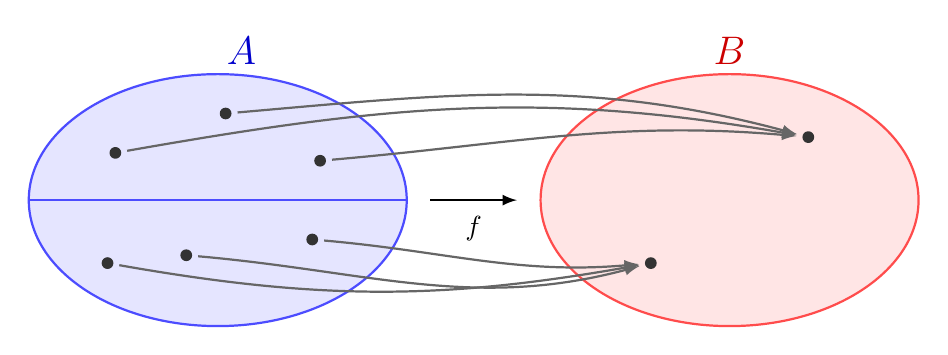
\begin{tikzpicture}[>=latex]

% --- Global TikZ Styles for Consistency ---
\tikzset{
    setA/.style={fill=blue!10, draw=blue!70, thick},
    setB/.style={fill=red!10, draw=red!70, thick},
    labelA/.style={text=blue!80!black, font=\Large\bfseries},
    labelB/.style={text=red!80!black, font=\Large\bfseries},
    point/.style={circle, fill=black!80, inner sep=1.5pt},
    arrow/.style={->, >=latex, thick, draw=black!60, shorten >=2pt, shorten <=2pt}
}

    % Verzameling A
    \path[setA] (0, 0) ellipse (2.4cm and 1.6cm);
    \node[labelA] at (0.3, 1.9) {$A$};
    
    % Horizontale scheidingslijn in A
    \draw[draw=blue!70, thick] (-2.4, 0) -- (2.4, 0);

    % Punten in bovenste helft van A
    \node[point] (a1) at (-1.3, 0.6) {};
    \node[point] (a2) at (0.1, 1.1) {};
    \node[point] (a3) at (1.3, 0.5) {};

    % Punten in onderste helft van A
    \node[point] (a4) at (-1.4, -0.8) {};
    \node[point] (a5) at (-0.4, -0.7) {};
    \node[point] (a6) at (1.2, -0.5) {};

    % Verzameling B
    \path[setB] (6.5, 0) ellipse (2.4cm and 1.6cm);
    \node[labelB] at (6.5, 1.9) {$B$};

    % Punten in B
    \node[point] (b1) at (7.5, 0.8) {};
    \node[point] (b2) at (5.5, -0.8) {};

    % Functiepijl en label f in het midden
    \draw[->, >=latex, thick] (2.7, 0) -- (3.8, 0) node[midway, below=2pt] {$f$};

    % Pijlen van A naar B (bovenste helft)
    % De "out" en "in" hoeken zorgen voor de vloeiende curves
    \draw[arrow] (a1) to[out=10, in=170] (b1);
    \draw[arrow] (a2) to[out=5, in=165] (b1);
    \draw[arrow] (a3) to[out=5, in=175] (b1);

    % Pijlen van A naar B (onderste helft)
    \draw[arrow] (a4) to[out=-10, in=190] (b2);
    \draw[arrow] (a5) to[out=-5, in=195] (b2);
    \draw[arrow] (a6) to[out=-5, in=185] (b2);
    
\end{tikzpicture}